\documentclass{article}

\usepackage[utf8]{inputenc}
\usepackage[english]{babel}
\usepackage{xcolor,upquote,charter,graphicx}
\usepackage[hidelinks]{hyperref}
\usepackage[top=3cm, bottom=4cm, left=3cm, right=3.5cm]{geometry}
\usepackage{caption}

\usepackage{minted}
% \usemintedstyle{monokai}

\newcommand{\inlinecode}[1]{\mintinline{python}{#1}}
\newcommand{\link}[2]{\textcolor{blue}{\href{#2}{#1}}}
\newcommand{\question}[1]{\item[$\bullet$] 
	\begin{minipage}[t]{\textwidth}
		\bfseries#1
	\end{minipage}
	\hfil
}

\newenvironment{answer}{}{}
\newenvironment{faq}{\begin{description}}{\end{description}}

\definecolor{bg}{rgb}{0.95,0.95,0.95}

\setminted[python]
{
	mathescape,
	python3=true,
	tabsize=4,
	bgcolor=bg
}

\pagestyle{empty}

\captionsetup[table]{name=Listing}

\begin{document}
	
	\section*{\Huge6.00.1x Week 1 FAQ}
	
	\subsection*{\LARGE Commonly Used Acronyms}
	
	\begin{description}
		\item[PSETs] Problem Sets
		
		\item[Fexes] Finger Exercises
		
		\item[Community TAs/TAs] Community Teaching Assistants
	\end{description}
	
	\subsection*{\LARGE Course Logistics}
	
	\begin{faq}
		\question{Can I try the course before upgrading to a Verified Certificate\,?}
		\begin{answer}
			Of course! You are welcome to try the course and all its materials before
			upgrading to a verified certificate but if you wish to receive a certificate you
			must upgrade before the date indicated in the ``Home'' tab.
		\end{answer}
		
		\question{Are finger exercises graded\,?}
		\begin{answer}
			Yes, completing finger exercises counts towards your final grade but you
			have unlimited attempts to complete them. Finger exercises are here to help
			you solidify your knowledge and learn from your mistakes.
		\end{answer}
		
		\question{How many attempts am I allowed for finger exercises\,?}
		\begin{answer}
			As many as you need. Finger exercises are here to help you solidify your
			knowledge, detect areas where you need to work on and learn the topics
			presented.
		\end{answer}
		
		\question{Can I spend more time than the estimated time on an exercise\,?}
		\begin{answer}
			Absolutely! It’s okay to spend more than the estimated time on a finger
			exercise, just make sure that you understand the topic and what the exercise
			required you to do so you are able to solve it more quickly the next time you
			are presented with a similar challenge. If you have any questions on the
			exercises please ask them in the discussion forums. Your classmates and
			Community TAs will be there to help you.
		\end{answer}
		
		\question{Are there deadlines I need to meet to complete lectures and exercises\,?}
		\begin{answer}
			No, in this self-paced version of the course there are no deadlines for lectures
			and exercises but you must complete all assignments before the course
			ends. You can check this date on the ``Home'' tab.
		\end{answer}
		
		\question{How to submit code to the grader for exercises that ask me to \textcolor[HTML]{900090}{assume that variables are already declared} or \textcolor[HTML]{900090}{to not ask for user input}\,?}
		\begin{answer}
			Don't include the variable declaration (or the line which gets the user input) when you paste your code to the
			grader, remove that line from your code as in the example \textcolor{blue}{\ref{Code you run on your IDE to test your solution}} and \textcolor{blue}{\ref{Code submitted to the grader}}:
			
			\begin{table}[htb]
				\caption{Code you run on your IDE to test your solution}
				\label{Code you run on your IDE to test your solution}
				\begin{minted}[linenos=true,stripnl=false]{python}
				# your own test value
				num = 5
				# what you are asked to code
				if num != 6:
				print(num)  
				\end{minted}
			\end{table}
			
			\begin{table}[htb]
				\caption{Code submitted to the grader}
				\label{Code submitted to the grader}
				\begin{minted}[linenos=true, firstnumber=3]{python}
				# what you are asked to code
				if num != 6:
				print(num)
				
				\end{minted}
			\end{table}
		\end{answer}
		
		\question{How can I keep indentation consistent when I paste my code to the grader\,?}
		\begin{answer}
			It usually helps to use tabs instead of spaces to create indentation.
			If you are using Sublime Text as your Text Editor, highlight your code to check if you see
			these dots to the left of your indented code (see~\figurename\,\textcolor{blue}{\ref{Indentation using spaces in Sublime Text}}).
			
			\begin{figure}[htb]
				\centering
				\caption{Indentation using spaces in Sublime Text} \label{Indentation using spaces in Sublime Text}
				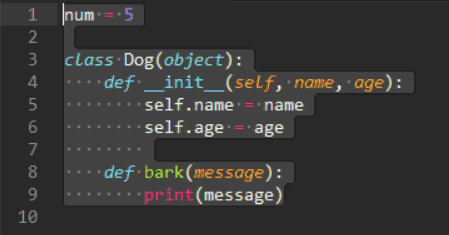
\includegraphics[scale=.5]{dots_indentation}
			\end{figure}
			
			If you do, this means that you are using spaces instead of tabs for
			indentation. To change this, select your code and click on the option highlighted with
			the red arrow on the image below, select the option located at the bottom right corner
			of the screen that says ``spaces'' (see~\figurename\,\textcolor{blue}{\ref{The spaces option}}).
			
			\begin{figure}[htb]
				\centering
				\caption{The \emph{spaces} option} \label{The spaces option}
				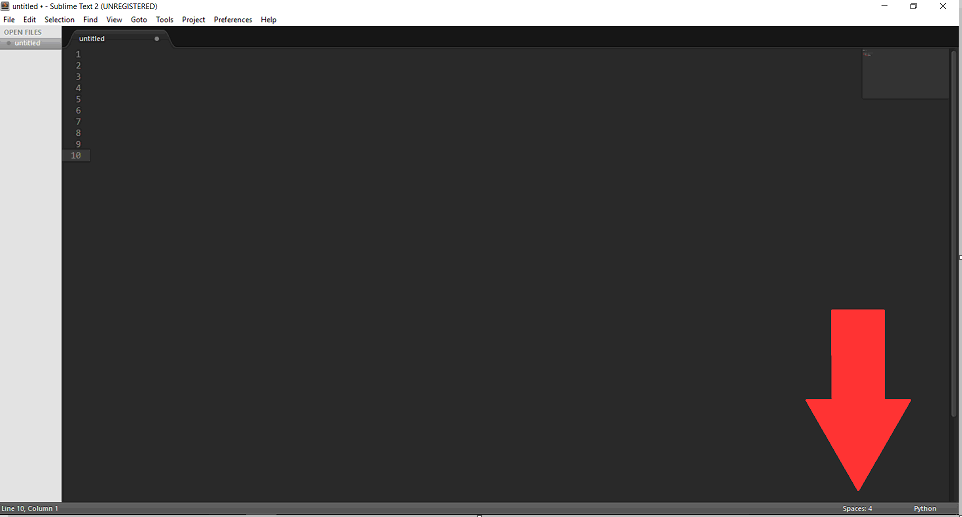
\includegraphics[scale=.25]{spaces_option}
			\end{figure}
			
			Then click on ``Convert Indentation to Tabs'' (see~\figurename\,\textcolor{blue}{\ref{Convert Indentation to Tabs}})
			
			\begin{figure}[htb]
				\centering
				\caption{Convert Indentation to Tabs} \label{Convert Indentation to Tabs}
				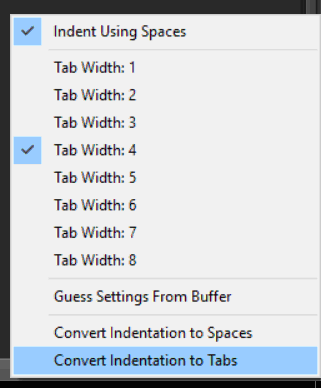
\includegraphics[scale=.5]{indentation_to_tabs}
			\end{figure}
			
			This will convert the spaces to tabs for the code you selected (see~\figurename\,\textcolor{blue}{\ref{Indentation using tabs in Sublime Text}}). After this you can copy and paste your code to the grader to keep your indentation. Good luck and
			if you have any questions we are here to help you in the discussions forums!
			
			\begin{figure}[htb]
				\centering
				\caption{Indentation using tabs in Sublime Text} \label{Indentation using tabs in Sublime Text}
				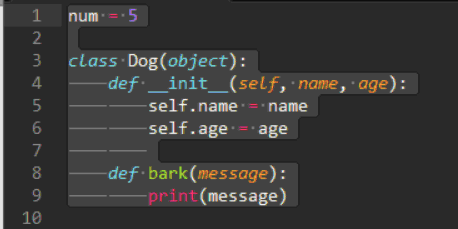
\includegraphics[scale=.5]{spaces_indentation}
			\end{figure}
		\end{answer}
	\end{faq}
	
	\clearpage
	
	\subsection*{\LARGE Course Content}
	
	\begin{faq}
		
		\question{What is Static Semantic vs. Semantic\,?}
		\begin{answer}
			Static semantics checks which syntactically correct expressions have
			meaning (e.g $3 \times 5$ is syntactically correct and multiplying two numbers has
			meaning) while Semantics interprets the meaning of the expression. That
			meaning can't be ambiguous.
		\end{answer}
		
		\question{Why is \inlinecode{True} different from true and \inlinecode{False} different from false in Python\,?}
		\begin{answer}
			Python is case sensitive; therefore the correct way to write Booleans is \inlinecode{True}
			and \inlinecode{False}. Using true and false will return an error because they are not
			recognized as Booleans.
		\end{answer}
		
		\question{What is Bool\,?}
		\begin{answer}
			Bool is a way to refer to Booleans, the truth values \inlinecode{True} and \inlinecode{False}.
		\end{answer}
		
		\question{Difference between $/$ and $//$ in Python}
		\begin{answer}
			The $/$ operator returns a \inlinecode{float}, while $//$ returns an \inlinecode{int}.
		\end{answer}
		
		\question{What does \inlinecode{!=} mean\,?}
		\begin{answer}
			This is a comparison operator that means ``not equal''. It returns \inlinecode{True} if the
			values compared are NOT equal and returns \inlinecode{False} if the values compared
			are equal.
		\end{answer}
		
		\question{What is the syntax for advanced string slicing\,?}
		\begin{answer}
			\inlinecode{"string"[start: end: step]}
		\end{answer}
		
		\question{Does \inlinecode{input()} always return a string\,?}
		\begin{answer}
			Yes. The Built-in function \inlinecode{input()} casts (``converts'') the input into a string and
			returns it. You can find more information on this function at \link{this link}{https://docs.python.org/3/library/functions.html\#input}.
		\end{answer}
		
		\question{What does the error ``\inlinecode{'str' object is not callable}'' mean\,?}
		\begin{answer}
			This error occurs when you name one of your variables \inlinecode{str}. If you use this
			name, you will ``replace'' the built-in function \inlinecode{str()} and you will not be able to
			use it anymore as a built-in function (More information on \inlinecode{str} at \link{this link}{https://docs.python.org/3/library/functions.html\#func-str}).
		\end{answer}
		
		\question{Difference between \inlinecode{if} and \inlinecode{elif}}
		\begin{answer}
			\inlinecode{if} is the first condition checked in an if/elif/else statement. If it is \inlinecode{True} the ``if'' code block will be executed. Else, if it is \inlinecode{False} the subsequent ``elif'' conditions will be checked. The code block of the first \inlinecode{elif} condition that evaluates to \inlinecode{True} will be executed. If none of them evaluates to \inlinecode{True}, the \inlinecode{else} code block will be automatically executed.
		\end{answer}
		
		\question{What is \# and what is it used for\,?}
		\begin{answer}
			In Python, \# is used to comment out a line of code or to add a comment to your code. These lines will not be executed as code, they are simply a way to help you explain your thought process to yourself and to other developers. For comments you do not need to follow the syntax of the programming language, you can write them as if you were talking to yourself or explaining what your code does. It is a very helpful way to communicate with developers that will look at your code in the future to try to understand how it works.
		\end{answer}
		
		\question{What is the difference between an Error and an Infinite Loop\,?}
		\begin{answer}
			An error is a warning thrown by your IDE or Shell, it is descriptive and gives
			you some information on what caused it. An infinite loop occurs when a while
			loop keeps executing indefinitely because there is no condition to stop its
			execution or if there is, that condition is never met. Infinite loops may not
			throw errors at all and the code will keep executing indefinitely until you
			manually execute a command to stop its execution.
		\end{answer}
		
		\question{How do I stop an infinite loop\,?}
		\begin{answer}
			By pressing \texttt{CTRL + C} on Windows.
		\end{answer}
		
		\question{Difference between While and For loop}
		\begin{answer}
			A While loop is used for situations where we want to keep executing a code
			block while a condition is not met, meaning that we don't know ahead of time
			how many times the loop has to be executed to meet that condition. In
			contrast, a For Loop is used when we do know how many times the loop has
			to be executed.
		\end{answer}
		
		\question{What is \inlinecode{str}\,?}
		\begin{answer}
			\inlinecode{str} is the built-in string class. You will learn about classes in the next few
			weeks of the course but right now you need to know that you can check if a
			variable is a string by comparing it directly to \inlinecode{str} (To learn more about \link{str}{https://docs.python.org/3/library/functions.html\#func-str})
		\end{answer}
		
		\question{Difference between \inlinecode{for i in} and \inlinecode{for i in range}\,?}
		\begin{answer}
			\inlinecode{for i in} is used to iterate over all the elements of a sequence (characters in a
			string, and elements of other data structures that you will learn in the next
			weeks of the course such as tuples and list). \inlinecode{for i in range} is a way to
			execute the loop a specific number of times that you can customize. Both
			update their variable (\inlinecode{i} in this case) on every loop iteration.
		\end{answer}
		
		\question{How does \inlinecode{while True} work?}
		\begin{answer}
			\inlinecode{while True} will execute a While loop indefinitely until it reaches a break
			statement to stop its execution. This is useful when you need to perform the
			same task an indefinite number of times until a condition is met.
		\end{answer}
		
	\end{faq}
	
\end{document}
